
\begin{figure}[h]        
    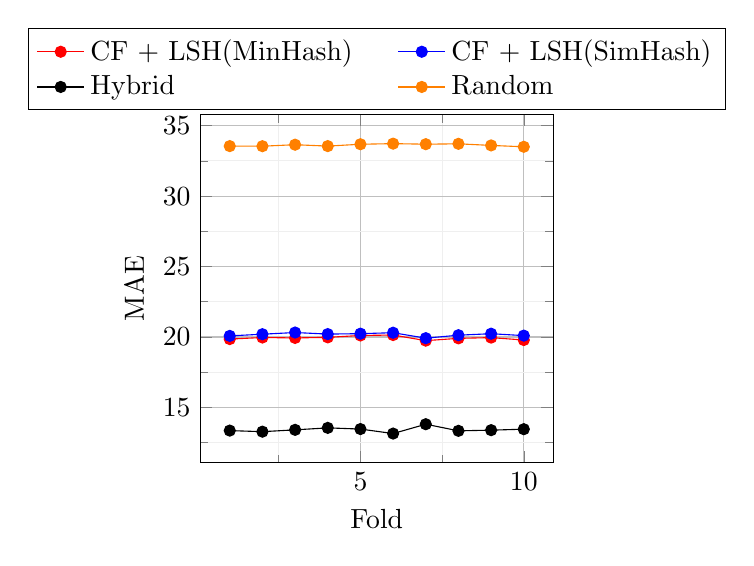
\begin{tikzpicture}
    \begin{axis}[
        xlabel=Fold,
        ylabel=MAE,
        height=6cm,
        width = 0.5*\textwidth,
        grid = both,
        minor tick num = 1,
        ytick={5,10,15,20,25,30,35,40,45,50},
        major grid style = {lightgray},
        minor grid style = {lightgray!25},
        legend cell align = {left},
        legend columns=2,
        legend style={/tikz/every even column/.append style={column sep=0.5cm}, at={(0.5,1.25)},anchor=north}
    ]
    
    % Add values and attributes for the first plot
    \addplot[color=red,mark=*] coordinates {
        (1,19.848849945235486)
        (2,19.960660825118655)
        (3,19.930649872216136)
        (4,19.971212121212123)
        (5,20.105969331872945)
        (6,20.135889010587807)
        (7,19.73783749246974)
        (8,19.901056974387995)
        (9,19.95312072144435)
        (10,19.782051516091933)
    };
    
    % Add values and attributes for the second plot
    \addplot[color=blue,mark=*] coordinates {
        (1,20.074917853231106)
        (2,20.195418035779483)
        (3,20.314439576487768)
        (4,20.203577948156262)
        (5,20.23340635268346)
        (6,20.30167944505294)
        (7,19.913744318078095)
        (8,20.125887657679037)
        (9,20.230635827598167)
        (10,20.094890377699482) 
    };

    \addplot[color=black,mark=*] coordinates {
        (1,13.352190580503834)
        (2,13.275319459656808)
        (3,13.405093099671413)
        (4,13.545198977729099)
        (5,13.461427528294998)
        (6,13.141493245710112)
        (7,13.805746727760638)
        (8,13.335091914784863)
        (9,13.382920462220923)
        (10,13.452436152540207)
    };

    \addplot[color=orange,mark=*] coordinates {
        (1,33.54850310332238)
        (2,33.54278933917488)
        (3,33.64786418400876)
        (4,33.54952537422417)
        (5,33.68105147864184)
        (6,33.723968601679445)
        (7,33.68522609029007)
        (8,33.71149528103835)
        (9,33.59780207743844)
        (10,33.5005567827087)
    };
    
    \legend{CF + LSH(MinHash), CF + LSH(SimHash), Hybrid, Random}
    \end{axis}
    \end{tikzpicture}
    \caption{\normalfont Mean absolute error measured on different folds of the synthetic dataset.}
    \label{fig:mae_synthetic}
\end{figure}
